\documentclass{article} % For LaTeX2e
\usepackage{iclr2022_conference,times}
% Optional math commands from https://github.com/goodfeli/dlbook_notation.
%%%%% NEW MATH DEFINITIONS %%%%%

\usepackage{amsmath,amsfonts,bm}

% Mark sections of captions for referring to divisions of figures
\newcommand{\figleft}{{\em (Left)}}
\newcommand{\figcenter}{{\em (Center)}}
\newcommand{\figright}{{\em (Right)}}
\newcommand{\figtop}{{\em (Top)}}
\newcommand{\figbottom}{{\em (Bottom)}}
\newcommand{\captiona}{{\em (a)}}
\newcommand{\captionb}{{\em (b)}}
\newcommand{\captionc}{{\em (c)}}
\newcommand{\captiond}{{\em (d)}}

% Highlight a newly defined term
\newcommand{\newterm}[1]{{\bf #1}}


% Figure reference, lower-case.
\def\figref#1{figure~\ref{#1}}
% Figure reference, capital. For start of sentence
\def\Figref#1{Figure~\ref{#1}}
\def\twofigref#1#2{figures \ref{#1} and \ref{#2}}
\def\quadfigref#1#2#3#4{figures \ref{#1}, \ref{#2}, \ref{#3} and \ref{#4}}
% Section reference, lower-case.
\def\secref#1{section~\ref{#1}}
% Section reference, capital.
\def\Secref#1{Section~\ref{#1}}
% Reference to two sections.
\def\twosecrefs#1#2{sections \ref{#1} and \ref{#2}}
% Reference to three sections.
\def\secrefs#1#2#3{sections \ref{#1}, \ref{#2} and \ref{#3}}
% Reference to an equation, lower-case.
\def\eqref#1{equation~\ref{#1}}
% Reference to an equation, upper case
\def\Eqref#1{Equation~\ref{#1}}
% A raw reference to an equation---avoid using if possible
\def\plaineqref#1{\ref{#1}}
% Reference to a chapter, lower-case.
\def\chapref#1{chapter~\ref{#1}}
% Reference to an equation, upper case.
\def\Chapref#1{Chapter~\ref{#1}}
% Reference to a range of chapters
\def\rangechapref#1#2{chapters\ref{#1}--\ref{#2}}
% Reference to an algorithm, lower-case.
\def\algref#1{algorithm~\ref{#1}}
% Reference to an algorithm, upper case.
\def\Algref#1{Algorithm~\ref{#1}}
\def\twoalgref#1#2{algorithms \ref{#1} and \ref{#2}}
\def\Twoalgref#1#2{Algorithms \ref{#1} and \ref{#2}}
% Reference to a part, lower case
\def\partref#1{part~\ref{#1}}
% Reference to a part, upper case
\def\Partref#1{Part~\ref{#1}}
\def\twopartref#1#2{parts \ref{#1} and \ref{#2}}

\def\ceil#1{\lceil #1 \rceil}
\def\floor#1{\lfloor #1 \rfloor}
\def\1{\bm{1}}
\newcommand{\train}{\mathcal{D}}
\newcommand{\valid}{\mathcal{D_{\mathrm{valid}}}}
\newcommand{\test}{\mathcal{D_{\mathrm{test}}}}

\def\eps{{\epsilon}}


% Random variables
\def\reta{{\textnormal{$\eta$}}}
\def\ra{{\textnormal{a}}}
\def\rb{{\textnormal{b}}}
\def\rc{{\textnormal{c}}}
\def\rd{{\textnormal{d}}}
\def\re{{\textnormal{e}}}
\def\rf{{\textnormal{f}}}
\def\rg{{\textnormal{g}}}
\def\rh{{\textnormal{h}}}
\def\ri{{\textnormal{i}}}
\def\rj{{\textnormal{j}}}
\def\rk{{\textnormal{k}}}
\def\rl{{\textnormal{l}}}
% rm is already a command, just don't name any random variables m
\def\rn{{\textnormal{n}}}
\def\ro{{\textnormal{o}}}
\def\rp{{\textnormal{p}}}
\def\rq{{\textnormal{q}}}
\def\rr{{\textnormal{r}}}
\def\rs{{\textnormal{s}}}
\def\rt{{\textnormal{t}}}
\def\ru{{\textnormal{u}}}
\def\rv{{\textnormal{v}}}
\def\rw{{\textnormal{w}}}
\def\rx{{\textnormal{x}}}
\def\ry{{\textnormal{y}}}
\def\rz{{\textnormal{z}}}

% Random vectors
\def\rvepsilon{{\mathbf{\epsilon}}}
\def\rvtheta{{\mathbf{\theta}}}
\def\rva{{\mathbf{a}}}
\def\rvb{{\mathbf{b}}}
\def\rvc{{\mathbf{c}}}
\def\rvd{{\mathbf{d}}}
\def\rve{{\mathbf{e}}}
\def\rvf{{\mathbf{f}}}
\def\rvg{{\mathbf{g}}}
\def\rvh{{\mathbf{h}}}
\def\rvu{{\mathbf{i}}}
\def\rvj{{\mathbf{j}}}
\def\rvk{{\mathbf{k}}}
\def\rvl{{\mathbf{l}}}
\def\rvm{{\mathbf{m}}}
\def\rvn{{\mathbf{n}}}
\def\rvo{{\mathbf{o}}}
\def\rvp{{\mathbf{p}}}
\def\rvq{{\mathbf{q}}}
\def\rvr{{\mathbf{r}}}
\def\rvs{{\mathbf{s}}}
\def\rvt{{\mathbf{t}}}
\def\rvu{{\mathbf{u}}}
\def\rvv{{\mathbf{v}}}
\def\rvw{{\mathbf{w}}}
\def\rvx{{\mathbf{x}}}
\def\rvy{{\mathbf{y}}}
\def\rvz{{\mathbf{z}}}

% Elements of random vectors
\def\erva{{\textnormal{a}}}
\def\ervb{{\textnormal{b}}}
\def\ervc{{\textnormal{c}}}
\def\ervd{{\textnormal{d}}}
\def\erve{{\textnormal{e}}}
\def\ervf{{\textnormal{f}}}
\def\ervg{{\textnormal{g}}}
\def\ervh{{\textnormal{h}}}
\def\ervi{{\textnormal{i}}}
\def\ervj{{\textnormal{j}}}
\def\ervk{{\textnormal{k}}}
\def\ervl{{\textnormal{l}}}
\def\ervm{{\textnormal{m}}}
\def\ervn{{\textnormal{n}}}
\def\ervo{{\textnormal{o}}}
\def\ervp{{\textnormal{p}}}
\def\ervq{{\textnormal{q}}}
\def\ervr{{\textnormal{r}}}
\def\ervs{{\textnormal{s}}}
\def\ervt{{\textnormal{t}}}
\def\ervu{{\textnormal{u}}}
\def\ervv{{\textnormal{v}}}
\def\ervw{{\textnormal{w}}}
\def\ervx{{\textnormal{x}}}
\def\ervy{{\textnormal{y}}}
\def\ervz{{\textnormal{z}}}

% Random matrices
\def\rmA{{\mathbf{A}}}
\def\rmB{{\mathbf{B}}}
\def\rmC{{\mathbf{C}}}
\def\rmD{{\mathbf{D}}}
\def\rmE{{\mathbf{E}}}
\def\rmF{{\mathbf{F}}}
\def\rmG{{\mathbf{G}}}
\def\rmH{{\mathbf{H}}}
\def\rmI{{\mathbf{I}}}
\def\rmJ{{\mathbf{J}}}
\def\rmK{{\mathbf{K}}}
\def\rmL{{\mathbf{L}}}
\def\rmM{{\mathbf{M}}}
\def\rmN{{\mathbf{N}}}
\def\rmO{{\mathbf{O}}}
\def\rmP{{\mathbf{P}}}
\def\rmQ{{\mathbf{Q}}}
\def\rmR{{\mathbf{R}}}
\def\rmS{{\mathbf{S}}}
\def\rmT{{\mathbf{T}}}
\def\rmU{{\mathbf{U}}}
\def\rmV{{\mathbf{V}}}
\def\rmW{{\mathbf{W}}}
\def\rmX{{\mathbf{X}}}
\def\rmY{{\mathbf{Y}}}
\def\rmZ{{\mathbf{Z}}}

% Elements of random matrices
\def\ermA{{\textnormal{A}}}
\def\ermB{{\textnormal{B}}}
\def\ermC{{\textnormal{C}}}
\def\ermD{{\textnormal{D}}}
\def\ermE{{\textnormal{E}}}
\def\ermF{{\textnormal{F}}}
\def\ermG{{\textnormal{G}}}
\def\ermH{{\textnormal{H}}}
\def\ermI{{\textnormal{I}}}
\def\ermJ{{\textnormal{J}}}
\def\ermK{{\textnormal{K}}}
\def\ermL{{\textnormal{L}}}
\def\ermM{{\textnormal{M}}}
\def\ermN{{\textnormal{N}}}
\def\ermO{{\textnormal{O}}}
\def\ermP{{\textnormal{P}}}
\def\ermQ{{\textnormal{Q}}}
\def\ermR{{\textnormal{R}}}
\def\ermS{{\textnormal{S}}}
\def\ermT{{\textnormal{T}}}
\def\ermU{{\textnormal{U}}}
\def\ermV{{\textnormal{V}}}
\def\ermW{{\textnormal{W}}}
\def\ermX{{\textnormal{X}}}
\def\ermY{{\textnormal{Y}}}
\def\ermZ{{\textnormal{Z}}}

% Vectors
\def\vzero{{\bm{0}}}
\def\vone{{\bm{1}}}
\def\vmu{{\bm{\mu}}}
\def\vtheta{{\bm{\theta}}}
\def\va{{\bm{a}}}
\def\vb{{\bm{b}}}
\def\vc{{\bm{c}}}
\def\vd{{\bm{d}}}
\def\ve{{\bm{e}}}
\def\vf{{\bm{f}}}
\def\vg{{\bm{g}}}
\def\vh{{\bm{h}}}
\def\vi{{\bm{i}}}
\def\vj{{\bm{j}}}
\def\vk{{\bm{k}}}
\def\vl{{\bm{l}}}
\def\vm{{\bm{m}}}
\def\vn{{\bm{n}}}
\def\vo{{\bm{o}}}
\def\vp{{\bm{p}}}
\def\vq{{\bm{q}}}
\def\vr{{\bm{r}}}
\def\vs{{\bm{s}}}
\def\vt{{\bm{t}}}
\def\vu{{\bm{u}}}
\def\vv{{\bm{v}}}
\def\vw{{\bm{w}}}
\def\vx{{\bm{x}}}
\def\vy{{\bm{y}}}
\def\vz{{\bm{z}}}

% Elements of vectors
\def\evalpha{{\alpha}}
\def\evbeta{{\beta}}
\def\evepsilon{{\epsilon}}
\def\evlambda{{\lambda}}
\def\evomega{{\omega}}
\def\evmu{{\mu}}
\def\evpsi{{\psi}}
\def\evsigma{{\sigma}}
\def\evtheta{{\theta}}
\def\eva{{a}}
\def\evb{{b}}
\def\evc{{c}}
\def\evd{{d}}
\def\eve{{e}}
\def\evf{{f}}
\def\evg{{g}}
\def\evh{{h}}
\def\evi{{i}}
\def\evj{{j}}
\def\evk{{k}}
\def\evl{{l}}
\def\evm{{m}}
\def\evn{{n}}
\def\evo{{o}}
\def\evp{{p}}
\def\evq{{q}}
\def\evr{{r}}
\def\evs{{s}}
\def\evt{{t}}
\def\evu{{u}}
\def\evv{{v}}
\def\evw{{w}}
\def\evx{{x}}
\def\evy{{y}}
\def\evz{{z}}

% Matrix
\def\mA{{\bm{A}}}
\def\mB{{\bm{B}}}
\def\mC{{\bm{C}}}
\def\mD{{\bm{D}}}
\def\mE{{\bm{E}}}
\def\mF{{\bm{F}}}
\def\mG{{\bm{G}}}
\def\mH{{\bm{H}}}
\def\mI{{\bm{I}}}
\def\mJ{{\bm{J}}}
\def\mK{{\bm{K}}}
\def\mL{{\bm{L}}}
\def\mM{{\bm{M}}}
\def\mN{{\bm{N}}}
\def\mO{{\bm{O}}}
\def\mP{{\bm{P}}}
\def\mQ{{\bm{Q}}}
\def\mR{{\bm{R}}}
\def\mS{{\bm{S}}}
\def\mT{{\bm{T}}}
\def\mU{{\bm{U}}}
\def\mV{{\bm{V}}}
\def\mW{{\bm{W}}}
\def\mX{{\bm{X}}}
\def\mY{{\bm{Y}}}
\def\mZ{{\bm{Z}}}
\def\mBeta{{\bm{\beta}}}
\def\mPhi{{\bm{\Phi}}}
\def\mLambda{{\bm{\Lambda}}}
\def\mSigma{{\bm{\Sigma}}}

% Tensor
\DeclareMathAlphabet{\mathsfit}{\encodingdefault}{\sfdefault}{m}{sl}
\SetMathAlphabet{\mathsfit}{bold}{\encodingdefault}{\sfdefault}{bx}{n}
\newcommand{\tens}[1]{\bm{\mathsfit{#1}}}
\def\tA{{\tens{A}}}
\def\tB{{\tens{B}}}
\def\tC{{\tens{C}}}
\def\tD{{\tens{D}}}
\def\tE{{\tens{E}}}
\def\tF{{\tens{F}}}
\def\tG{{\tens{G}}}
\def\tH{{\tens{H}}}
\def\tI{{\tens{I}}}
\def\tJ{{\tens{J}}}
\def\tK{{\tens{K}}}
\def\tL{{\tens{L}}}
\def\tM{{\tens{M}}}
\def\tN{{\tens{N}}}
\def\tO{{\tens{O}}}
\def\tP{{\tens{P}}}
\def\tQ{{\tens{Q}}}
\def\tR{{\tens{R}}}
\def\tS{{\tens{S}}}
\def\tT{{\tens{T}}}
\def\tU{{\tens{U}}}
\def\tV{{\tens{V}}}
\def\tW{{\tens{W}}}
\def\tX{{\tens{X}}}
\def\tY{{\tens{Y}}}
\def\tZ{{\tens{Z}}}


% Graph
\def\gA{{\mathcal{A}}}
\def\gB{{\mathcal{B}}}
\def\gC{{\mathcal{C}}}
\def\gD{{\mathcal{D}}}
\def\gE{{\mathcal{E}}}
\def\gF{{\mathcal{F}}}
\def\gG{{\mathcal{G}}}
\def\gH{{\mathcal{H}}}
\def\gI{{\mathcal{I}}}
\def\gJ{{\mathcal{J}}}
\def\gK{{\mathcal{K}}}
\def\gL{{\mathcal{L}}}
\def\gM{{\mathcal{M}}}
\def\gN{{\mathcal{N}}}
\def\gO{{\mathcal{O}}}
\def\gP{{\mathcal{P}}}
\def\gQ{{\mathcal{Q}}}
\def\gR{{\mathcal{R}}}
\def\gS{{\mathcal{S}}}
\def\gT{{\mathcal{T}}}
\def\gU{{\mathcal{U}}}
\def\gV{{\mathcal{V}}}
\def\gW{{\mathcal{W}}}
\def\gX{{\mathcal{X}}}
\def\gY{{\mathcal{Y}}}
\def\gZ{{\mathcal{Z}}}

% Sets
\def\sA{{\mathbb{A}}}
\def\sB{{\mathbb{B}}}
\def\sC{{\mathbb{C}}}
\def\sD{{\mathbb{D}}}
% Don't use a set called E, because this would be the same as our symbol
% for expectation.
\def\sF{{\mathbb{F}}}
\def\sG{{\mathbb{G}}}
\def\sH{{\mathbb{H}}}
\def\sI{{\mathbb{I}}}
\def\sJ{{\mathbb{J}}}
\def\sK{{\mathbb{K}}}
\def\sL{{\mathbb{L}}}
\def\sM{{\mathbb{M}}}
\def\sN{{\mathbb{N}}}
\def\sO{{\mathbb{O}}}
\def\sP{{\mathbb{P}}}
\def\sQ{{\mathbb{Q}}}
\def\sR{{\mathbb{R}}}
\def\sS{{\mathbb{S}}}
\def\sT{{\mathbb{T}}}
\def\sU{{\mathbb{U}}}
\def\sV{{\mathbb{V}}}
\def\sW{{\mathbb{W}}}
\def\sX{{\mathbb{X}}}
\def\sY{{\mathbb{Y}}}
\def\sZ{{\mathbb{Z}}}

% Entries of a matrix
\def\emLambda{{\Lambda}}
\def\emA{{A}}
\def\emB{{B}}
\def\emC{{C}}
\def\emD{{D}}
\def\emE{{E}}
\def\emF{{F}}
\def\emG{{G}}
\def\emH{{H}}
\def\emI{{I}}
\def\emJ{{J}}
\def\emK{{K}}
\def\emL{{L}}
\def\emM{{M}}
\def\emN{{N}}
\def\emO{{O}}
\def\emP{{P}}
\def\emQ{{Q}}
\def\emR{{R}}
\def\emS{{S}}
\def\emT{{T}}
\def\emU{{U}}
\def\emV{{V}}
\def\emW{{W}}
\def\emX{{X}}
\def\emY{{Y}}
\def\emZ{{Z}}
\def\emSigma{{\Sigma}}

% entries of a tensor
% Same font as tensor, without \bm wrapper
\newcommand{\etens}[1]{\mathsfit{#1}}
\def\etLambda{{\etens{\Lambda}}}
\def\etA{{\etens{A}}}
\def\etB{{\etens{B}}}
\def\etC{{\etens{C}}}
\def\etD{{\etens{D}}}
\def\etE{{\etens{E}}}
\def\etF{{\etens{F}}}
\def\etG{{\etens{G}}}
\def\etH{{\etens{H}}}
\def\etI{{\etens{I}}}
\def\etJ{{\etens{J}}}
\def\etK{{\etens{K}}}
\def\etL{{\etens{L}}}
\def\etM{{\etens{M}}}
\def\etN{{\etens{N}}}
\def\etO{{\etens{O}}}
\def\etP{{\etens{P}}}
\def\etQ{{\etens{Q}}}
\def\etR{{\etens{R}}}
\def\etS{{\etens{S}}}
\def\etT{{\etens{T}}}
\def\etU{{\etens{U}}}
\def\etV{{\etens{V}}}
\def\etW{{\etens{W}}}
\def\etX{{\etens{X}}}
\def\etY{{\etens{Y}}}
\def\etZ{{\etens{Z}}}

% The true underlying data generating distribution
\newcommand{\pdata}{p_{\rm{data}}}
% The empirical distribution defined by the training set
\newcommand{\ptrain}{\hat{p}_{\rm{data}}}
\newcommand{\Ptrain}{\hat{P}_{\rm{data}}}
% The model distribution
\newcommand{\pmodel}{p_{\rm{model}}}
\newcommand{\Pmodel}{P_{\rm{model}}}
\newcommand{\ptildemodel}{\tilde{p}_{\rm{model}}}
% Stochastic autoencoder distributions
\newcommand{\pencode}{p_{\rm{encoder}}}
\newcommand{\pdecode}{p_{\rm{decoder}}}
\newcommand{\precons}{p_{\rm{reconstruct}}}

\newcommand{\laplace}{\mathrm{Laplace}} % Laplace distribution

\newcommand{\E}{\mathbb{E}}
\newcommand{\Ls}{\mathcal{L}}
\newcommand{\R}{\mathbb{R}}
\newcommand{\emp}{\tilde{p}}
\newcommand{\lr}{\alpha}
\newcommand{\reg}{\lambda}
\newcommand{\rect}{\mathrm{rectifier}}
\newcommand{\softmax}{\mathrm{softmax}}
\newcommand{\sigmoid}{\sigma}
\newcommand{\softplus}{\zeta}
\newcommand{\KL}{D_{\mathrm{KL}}}
\newcommand{\Var}{\mathrm{Var}}
\newcommand{\standarderror}{\mathrm{SE}}
\newcommand{\Cov}{\mathrm{Cov}}
% Wolfram Mathworld says $L^2$ is for function spaces and $\ell^2$ is for vectors
% But then they seem to use $L^2$ for vectors throughout the site, and so does
% wikipedia.
\newcommand{\normlzero}{L^0}
\newcommand{\normlone}{L^1}
\newcommand{\normltwo}{L^2}
\newcommand{\normlp}{L^p}
\newcommand{\normmax}{L^\infty}

\newcommand{\parents}{Pa} % See usage in notation.tex. Chosen to match Daphne's book.

\DeclareMathOperator*{\argmax}{arg\,max}
\DeclareMathOperator*{\argmin}{arg\,min}

\DeclareMathOperator{\sign}{sign}
\DeclareMathOperator{\Tr}{Tr}
\let\ab\allowbreak


%######## APS360: Uncomment your submission name
\newcommand{\apsname}{Project Progress Report}
%\newcommand{\apsname}{Progress Report}
%\newcommand{\apsname}{Final Report}

%######## APS360: Put your Group Number here
\newcommand{\gpnumber}{4}

\usepackage{hyperref}
\usepackage{url}
\usepackage{graphicx}
\usepackage{float}
\usepackage{caption} 
\restylefloat{table}

%######## APS360: Put your project Title here
\title{Progress Report: AUTONOMOUS CAR USING CNN\\}


%######## APS360: Put your names, student IDs and Emails here
\author{Rudra Dey  \\
Student\# 1010124866\\
\texttt{rudra.dey@mail.utoronto.ca } \\
\And
Pravin Kalaivannan  \\
Student\# 1010141295 \\ 
\texttt{pravin.kalaivannan@mail.utoronto.ca} \\
\AND
Aadavan Vasudevan  \\
Student\# 1010101514 \\
\texttt{aadavan.vasudevan@mail.utoronto.ca} \\
\And
Abishan Baheerathan \\
Student\# 1010218756 \\
\texttt{abishan.baheerathan@mail.utoronto.ca} \\
\AND
}

% The \author macro works with any number of authors. There are two commands
% used to separate the names and addresses of multiple authors: \And and \AND.
%
% Using \And between authors leaves it to \LaTeX{} to determine where to break
% the lines. Using \AND forces a linebreak at that point. So, if \LaTeX{}
% puts 3 of 4 authors names on the first line, and the last on the second
% line, try using \AND instead of \And before the third author name.

\newcommand{\fix}{\marginpar{FIX}}
\newcommand{\new}{\marginpar{NEW}}

\iclrfinalcopy 
%######## APS360: Document starts here
\begin{document}

\maketitle

\begin{abstract}
This document presents our team’s progress in developing an autonomous car. The project description contains minor changes that we made and explains why deep learning is necessary for this project. The team’s responsibilities, work completed, and a future timeline are listed, which also provides solutions to redundancies. The data processing section discusses how the team collects data from the simulator to create a dataset and how that data is modified to use on the CNN model. This document compares a baseline model to our primary model and shows the quantitative results that we collected. 
\\
%######## APS360: Do not change the next line. This shows your Main body page count.
Total Pages: \pageref{last_page}
\end{abstract}

\section{Project Description}

This project involves training a simulated autonomous car using a convolutional neural network (CNN) and a forward-facing camera. The goal of this project is to build a model that can predict steering commands based on visual input from the camera. This should allow the car to drive on its own without the need for additional sensors or manual commands.  

Our team’s motivation behind the project was to explore a simplified, small-scale version of autonomous driving systems, using deep learning. Furthermore, traditional rule-based approaches are limited by their inability to predict the vast number of driving scenarios that can occur. Deep learning offers the ability to learn from data and generalize across different visual conditions. This made it a suitable choice for handling the complex input from a moving car. The project also provided insight into the effectiveness of vision-only autonomous systems and the role of deep learning in embedded robotics.


\section{Individual Contributions and Responsibilities}

Our team worked collaboratively throughout the project with clear task divisions and weekly milestones. All communication was handled through Discord, where we maintained an active group chat with frequent updates and responses. We held two scheduled meetings every week and used GitHub to track code progress, manage issues, and handle version control across all components. The team has a shared Google Drive where documents are added for collaboration. 


\subsection{Individual Contributions}
Each team member was assigned specific responsibilities:

\begin{itemize}
  \item \textbf{Aadavan} handled the baseline rule-based model used for comparison, authored the ethical considerations section, and participated in model evaluation. Additionally, helped build the CNN architecture.

  \item \textbf{Rudra} led the software and simulator setup (camera system), collected the training dataset, and worked on preprocessing the image data. Helped with model training and tuning. 

  \item \textbf{Pravin} contributed to background research on similar projects and helped build the CNN architecture. Additionally, helped create the dataset using CARLA along with a training regime.

  \item \textbf{Abishan} supported data preprocessing, designed the training setup (optimizer, loss function, hyperparameters), created the project's risk register, and contributed to model training.
\end{itemize}

\subsection{Timeline of Completed Tasks}

We maintained an internal task schedule which helped the team stay on track. Table~\ref{tab:currentTimeline} summarizes the tasks completed by each team member, their completion dates, and the outcomes of each task.

\begin{table}[h!]
\centering
\caption{Timeline of all completed tasks}
\begin{tabular}{|p{2.5cm}|p{3cm}|p{3cm}|p{5.5cm}|}
\hline
\textbf{Task} & \textbf{Team Members} & \textbf{Completion Date} & \textbf{Result} \\
\hline
Brainstorm Project Ideas & All Members & June 9, 2025 & Team decided to work on a simulated autonomous car \\
\hline
Model Selection & All Members & June 10, 2025 & Team decided on using a CNN model \\
\hline
Project Proposal (Draft \& Final) & All Members & June 12--13, 2025 & Completed a Project Proposal document \\
\hline
Data Collection \& Setup & Rudra, Aadavan, Pravin & June 20, 2025 & Team successfully set up CARLA simulator and collected data \\
\hline
Data Preprocessing & Rudra, Abishan & June 27, 2025 & Resized and normalized the image \\
\hline
Baseline Model Implementation & Aadavan & June 30, 2025 & Implemented ridge regression algorithm to create the baseline model \\
\hline
Architecture \& Model Building & Pravin, Aadavan & July 4, 2025 & Created a CNN architecture, to apply transfer learning \\
\hline
Training Regime Development & Abishan, Pravin & July 8, 2025 & Selecting appropirate training parameters \\
\hline
Model Training \& Tuning & Abishan, Rudra & July 10, 2025 & Trained model through a training dataset, adjusted overfitting, and quantified results \\
\hline
Progress Report & All Members & July 11, 2025 & Summarized work done so far, completed a progress report document \\
\hline
\end{tabular}
\label{tab:currentTimeline}
\end{table}

\subsection{Future Task Timeline and Responsibilities}

Table~\ref{tab:futureTimeline} outlines the tasks to be completed in the next phase of the project.

\begin{table}[H]
\centering
\caption{Future timeline with redundancies}
\begin{tabular}{|p{2.5cm}|p{4cm}|p{4cm}|p{4cm}|}
\hline
\textbf{Task} & \textbf{Team Member / Deadline} & \textbf{Description} & \textbf{Solutions to Redundancies} \\
\hline
Model Evaluation \& Testing & Aadavan, Pravin (July 25, 2025) & Test trained model with live input, identify weaknesses, confusion matrix. & The model should be tested under the same conditions to ensure consistency. \\
\hline
Final Report (Draft) & Everyone (Aug 1, 2025) & Write first full draft including abstract, results, ethics, background, etc. & If an assigned section has not been started 2 days before the deadline, it will be redistributed. \\
\hline
Final Report (Final) & Everyone (Aug 8, 2025) & Submit the polished report with citations and final results. & Everyone is required to edit their section and must read through the entire document once. \\
\hline
Record Presentation & Everyone (Aug 12, 2025) & Record team sections, align visuals with speech. & Everyone will record their assigned section and upload to the shared drive to ensure all clips are collected. \\
\hline
Edit Presentation Video & Rudra, Pravin (Aug 13, 2025) & Merge clips, finalize cuts, add transitions, captions, or diagrams. & Rudra will be the primary editor; Pravin will take over if necessary. \\
\hline
Final Deliverable & Rudra (Aug 15, 2025) & Submit final code, data, report, and video via the course portal. & Rudra will be responsible for submitting all final work and verifying that it is satisfactory. \\
\hline
\end{tabular}
\label{tab:futureTimeline}
\end{table}

Each task was documented, versioned, and reviewed by at least one other team member. This structure helped us manage project risks, distribute workload evenly, and ensure consistent progress through each phase.

\section{Data Processing}

Data was collected from the CARLA simulator, including images and corresponding steering values. We then normalized the images allowing us to train our CNN.
Further, data augmentation was applied to increase the size and diversity of the dataset, leading to better generalization of the model.


\subsection{Data Collection and Cleaning}

In CARLA, some vehicles have autonomous functionality, which we used to collect data.
We attached an RGB Camera Sensor to the car to record 10 frames per second (FPS) as the car
travels around a designated map. In addition to the images, data for the steering values and turn signals of the car
were collected allowing for use as ground truth labels for training the model. This data collection was done on different maps with different weather conditions
to ensure a diverse dataset. We collected samples on three maps, in which the car collected data for 30 minutes, resulting in 54000 total images.


To clean the data, we removed any images that were all black, duplicates or not the correct resolution of 320x240 leaving us with 53457 images.  
The data is stored as numpy arrays, zipped and uploaded to a shared Google Colab file, ensuring access for all members. 

Procedure:
\begin{enumerate}
  \item{Spawn in a vehicle}
  \item{Attach an RGB Camera Sensor (front-facing) to the dash of the car.}
  \item{Collect image data (10 fps) along with steering data and turn signals.}
  \item {Clean the data by removing corrupted images and duplicates.}
  \item {Save the data as numpy arrays for easy access and processing.}
\end{enumerate}


\subsection{Data Preprocessing}
All collected images were resized to a resolution of 160x120 pixels as shown in Figure~\ref{fig:exampleofdataset}, with the pixel values normalized to a range of [0, 1]. 
This was done to ensure consistency in the input data, allowing the model to learn effectively from the images.

\begin{figure}[H] % h = here, t = top, b = bottom, p = page of floats
    \centering
    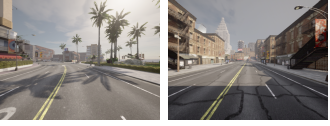
\includegraphics[width=0.6\textwidth]{exampleofdataset.png} % Adjust path and size
    \caption{Resized 3x160x120 example images from dataset}
    \label{fig:exampleofdataset}
\end{figure}



\subsection{Data Distribution}
We decided to do an 80/10/10 split for the training, validation and test sets respectively. This was done to ensure that we have a
large set of data for training, while also having enough data for validation and testing. Table 3 shows the distribution of the data.

\begin{table}[h]
\centering
\caption{Dataset Distribution}
\vspace{0.5em}
\begin{tabular}{|p{2cm}|p{2cm}|}
\hline
\textbf{Dataset Split} & \textbf{Total Images} \\ \hline
Training Set           & 42766 \\ \hline
Validation Set         & 5345 \\ \hline
Test Set               & 5346 \\ \hline
Total Images           & 53457  \\ \hline
\end{tabular}
\end{table}


\subsection{Data Agumentation}

Data augmentation was applied to the training set to increase the size and diversity of the dataset. We applied two techniques to generalize  the model and force
it to learn critical features. 

\begin{itemize}
  \item \textbf{Greyscale Conversion:} All training images were converted to greyscale reducing the the model's reliance on colour-based features, encouraging learning of more general visual features/road patterns. This will allow the model to improve, and work in different lighting conditions or if the camera is distorted.

  \item \textbf{Cutout Augmentation:} A rectangular region of each training image was masked out to simulate real-world situations (e.g. raindrop or debris on the camera lens). This encourages the model to learn relevant features from different parts of the image making it more robust overall. 
\end{itemize}

These augmentations lead to the training set being increased to 128298 images, with each image having two copies with each augmentations applied respectively as shown in Figure~\ref{fig:exampleofaugmented}.

\begin{figure}[H] % h = here, t = top, b = bottom, p = page of floats
    \centering
    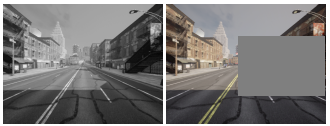
\includegraphics[width=0.6\textwidth]{exampleofaugmented.png} % Adjust path and size
    \caption{Augmented image examples (greyscale and cutout)}
    \label{fig:exampleofaugmented}
\end{figure}


\begin{table}[h]
\centering
\caption{Dataset Distribution after Training Set Augmentation}
\vspace{0.5em}
\begin{tabular}{|p{2cm}|p{2cm}|}
\hline
\textbf{Dataset Split} & \textbf{Total Images} \\ \hline
Training Set           & 42766 x 3 =  128298\\ \hline
Validation Set         & 5345 \\ \hline
Test Set               & 5346 \\ \hline
Total Images           & 138989 \\ \hline
\end{tabular}
\end{table}


\subsection{Plan for Testing on Unseen Data}

In order to evaluate the model's performance, we will be testing it on unseen data which we reserved 10\% of the dataset. Given how 
the data was collected sequentially across different maps and weather conditions, the test set will inherently contain frames that the model has not encountered before.
This will provide the model with different roads and turns to encounter and we can see how well it generalizes to new situations.

Additionally, to further test the model's generalization, we can load the model in CARLA and make it drive around a new map where data was not collected from, and see how well the model performs in 
real-time. This will allow us to visualize the model's performance and see how well it can adapt to new environments.

\subsection{Challenges Faced and Solutions}

During the data collection process, we faced several challenges and overcame them with the following solutions:

\begin{itemize}
  \item \textbf{Slow Initial Data Collection:} The simulator originally ran in real time, meaning that collecting data for 30 minitues would take that long in real time. 
  To solve this issue, we sped up the simulation, allowing us to collect data at a faster rate and collect more data in a shorter time frame.

  \item \textbf{Turn Signal Data Collection:} Collecting turn signal data was initially problematic, 
  because the vehicle's indicators were not being used by the automated vehicle in CARLA. 
  We tried to resolve this through manual activation based on steering angle, but this proved to be inaccurate and inconsistent. 
  We resolved this by enabling the CARLA Traffic Manager’s automatic lights, allowing turn signals to activate based on the vehicle's navigation. \
  In turn, this allows us to have accurate turn signal data for the training set. 

\end{itemize}
 
\section{Baseline Model}

Using a Ridge Regression Algorithm we created a baseline model that predicts steering angles for a self-driving car 
from grayscale camera images and turn signal inputs. This baseline model serves as a simple, interpretable baseline
such that we can compare our more complex primary neural network model later. To collect data, we used a simulator
called CARLA, to obtain camera images, turn signal inputs, and our ground truth label for the steering angles.


\subsection{Ridge Regression with Image Features}

In the model outlined in Figure~\ref{fig:diagram}, the grayscale images (of shape 160x120) were flattened into 1D feature vectors and normalized. The features themselves
represent the visual input of the car's front-facing camera. Additionally, left and right turning signals were captured as an
additional feature; combining this with our flattened grayscale images we were left with a numpy array of shape $N \times 19201$,
where $N$ represents the number of images, and 19201 are the number of feature column vectors. The Ridge Regression algorithm was
selected because it penalized large coefficients ($L_2$ norm), allowing for a generalized model. A series of models were trained
with different regularization strengths ($\alpha$), and the performance was evaluated using Mean Squared Error (MSE) and $R^2$ Score
on a held-out 20\% test set. 

\begin{figure}[H] % h = here, t = top, b = bottom, p = page of floats
    \centering
    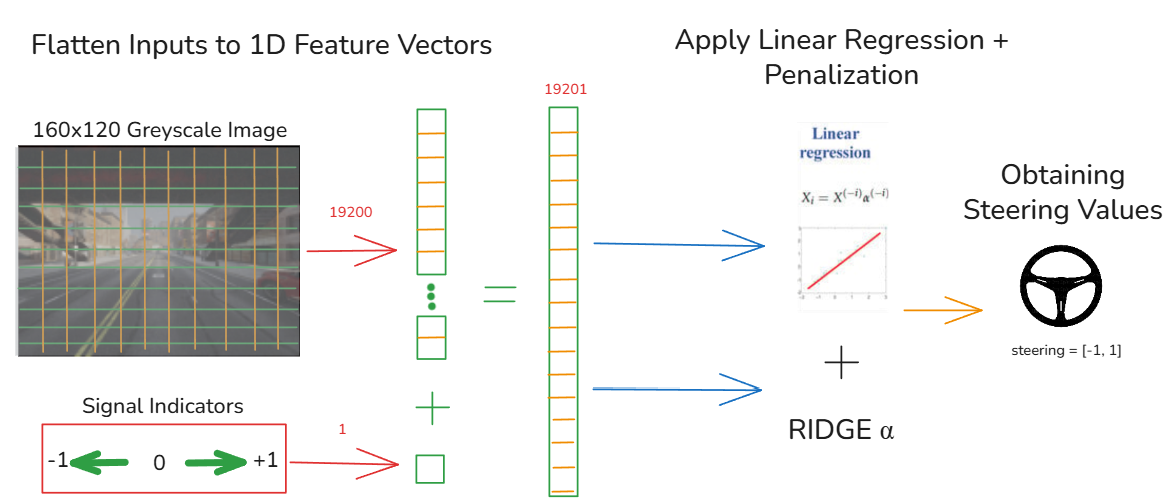
\includegraphics[width=1.0\textwidth]{diagram.png} % Adjust path and size
    \caption{Basic Architecture of Steering Angle Ridge Regrsession Model}
    \label{fig:diagram}
\end{figure}


\subsection{Minimal Tuning of $\alpha$}
The only hyperparameter needing to be tuned was the regularization strength for the Ridge Regression Algorithm. This was manually tuned,
and thus no validation set was used. A small set of candidate values for $\alpha$ was chosen: $\alpha \text{ } \epsilon \text{ } 
\{ 1, 10, 100, 250, 1000, 8000\}$ With each value of $\alpha$, the model was trained and tested with a dataset of 15 minutes of simulated
driving. By obtaining the average MSE and the average $R^2$ score, our fourth model of $\alpha = 100$ came out to be the best. 


\begin{figure}[H] % h = here, t = top, b = bottom, p = page of floats
    \centering
    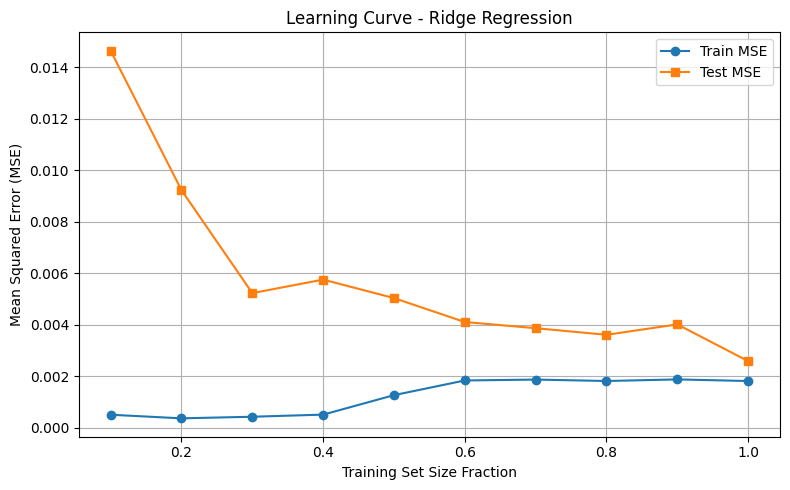
\includegraphics[width=0.6\textwidth]{model4learningcurve.png} % Adjust path and size
    \caption{This is the learning curve for "Model 4" a Ridge Regression Model with $\alpha = 100$}
    \label{fig:model4learningcurve}
\end{figure}

\subsection{Overfitting and Model Quality}
As shown in Figure~\ref{fig:model4learningcurve}, the results suggest some overfitting due to the model's tendency
to perform much better on training data than unseen data. This is reasonable since the training data frames, 
are all consecutive in nature, and the dataset used isn't extremely large either. In addition, as the training size
increases the gap between Test and Train MSEs narrows, suggesting that with more data the model will generalize better. 
The final test MSE is (~0.0025) which is quite low, meaning the model performs well overall after training on the data.


\subsection{Qualitative Observations}
When running the steering angle prediction model in the CARLA simulator, the model exhibited promising behaviour in terms of
autonomous driving capabilities, however with large limitations. The car was able to drive freely, using the model's predictions
from the front-facing grayscale camera images and turn signals provided by the user. In Figure~\ref{fig:model4demo} we can see 
the model taking a left turn in an intersection.

\begin{itemize}
  \item \textbf{Turn Signal Response:} The car consistently turned in the correct direction when prompted, showing that the model incorporated turn signal input effectively.

  \item \textbf{Obstacle Avoidance:} The vehicle generally avoided obstacles but occasionally clipped walls, suggesting basic spatial awareness but limited precision.

  \item \textbf{Lane-Keeping:} The car had trouble staying within lane boundaries, often drifting, especially during turns or on complex roads.

  \item \textbf{Map Generalization:} Despite limitations, the car performed reasonably well across different map layouts, showing decent control over turns.
\end{itemize}


\begin{figure}[H] % h = here, t = top, b = bottom, p = page of floats
    \centering
    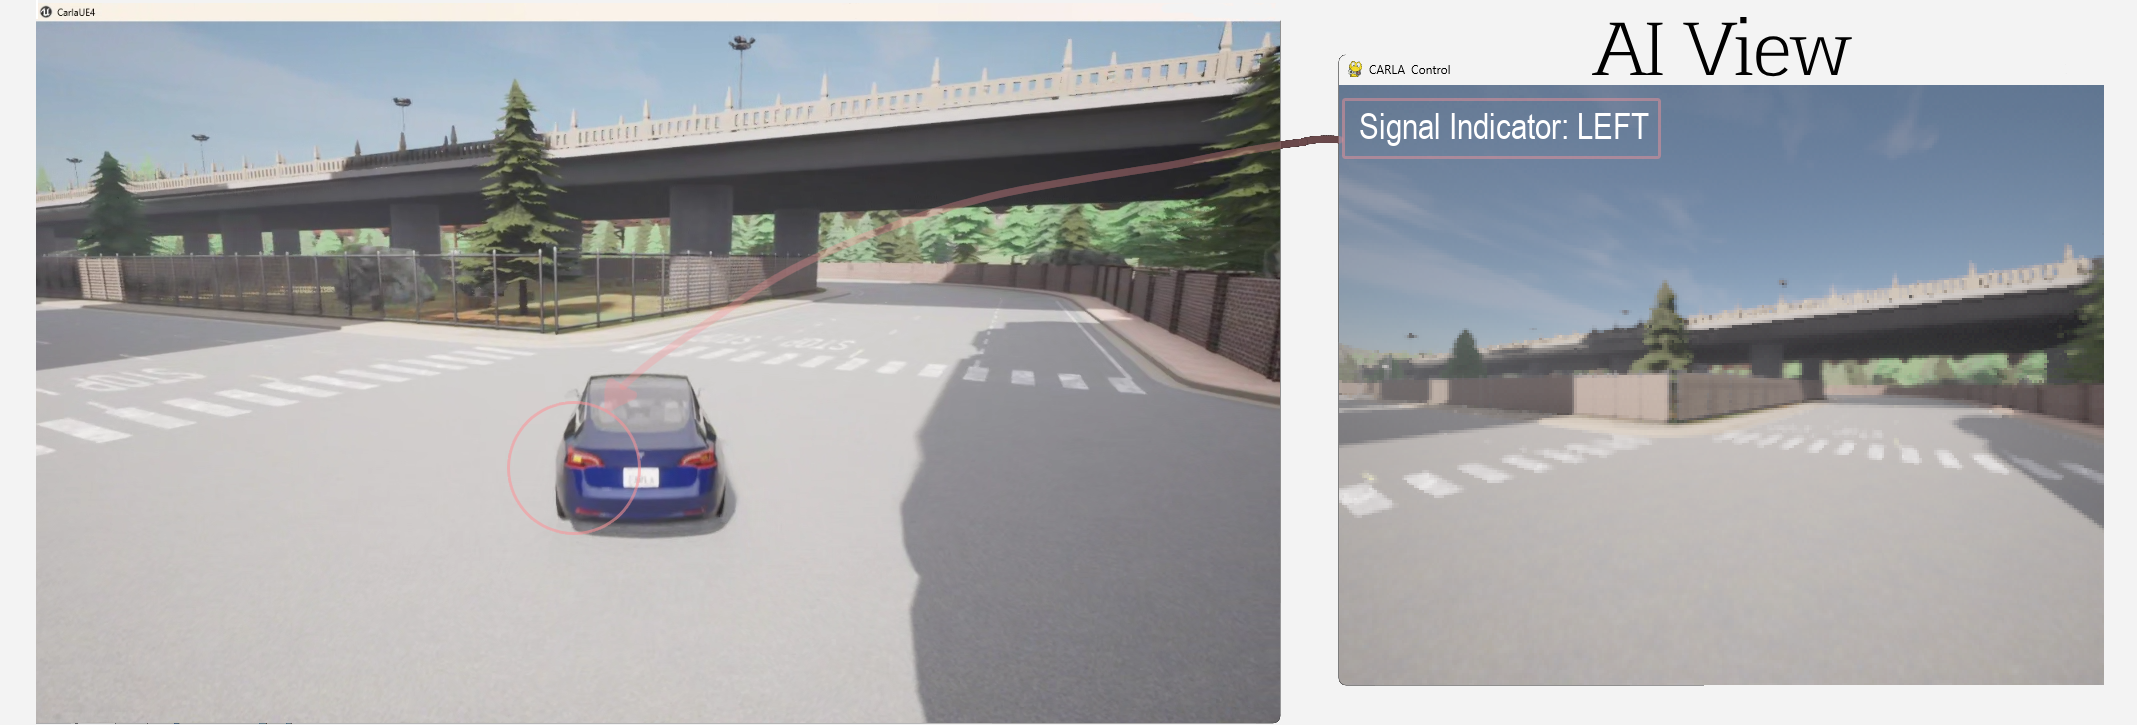
\includegraphics[width=1.0\textwidth]{model4demo.png} % Adjust path and size
    \caption{This is the demo for "Model 4" in CARLA}
    \label{fig:model4demo}
\end{figure}


\section{Primary Model}


\subsubsection{Transfer Learning with ResNet}

We opted to use transfer learning to take advantage of powerful visual feature extraction from pre-trained models, in this case we
used ResNet-18. This model was trained on ImageNet, and it has general-purpose feature extraction for RGB images. Rather than training
a convolutional neural network from scratch (which would require large amounts of labeled data and time). To use ResNet-18 we had 
removed its final classifcation layer which allowed us to reuse the learned convlutional layers for predicting the steering angles from 
the images themselves. By freezing the pretrained weights the model benefits from previous feature extraction and use it towards our dataset.

\subsubsection{Architecture Design}
The model architecture consists of two main components:
\begin{enumerate}
  \item Feature Extractor (ResNet-18)
    \begin{itemize}
      \item Input: RGB image resized to 224x224
      \item Output: 512-dimensional feature vector
      \item Final fully connected layer removed (cnn.fc = nn.Identity())
    \end{itemize}
  \item Prediction layer
    \begin{itemize}
      \item The extracted 512-dimensional image features are concatenated with a scalar turn signal input (left=-1, straight=0, right=1), forming a 513-dimensional input vector.
      \item This combined vector is passed through a small fully connected network:
      \begin{itemize}
        \item Linear(513 → 128) + ReLU activation
        \item Linear(128 → 1) for the final steering angle prediction
      \end{itemize}
    \end{itemize}
\end{enumerate}
\subsubsection{Training Methodology}
The model was trained using the following methodology:
\begin{itemize}
  \item Loss Function: Mean Squared Error (MSE) between predicted and ground truth steering angles.
  \item Optimizer: Adam optimizer with a learning rate of 1e-4, chosen for its robust adaptive learning capabilities.
  \item Batch Size: 32
  \item Epochs: 10
  \item Train/Validation Split: 80/20
\end{itemize}


\subsection{Model Performance}

Figure~\ref{fig:learningCurveforCNN} shows the learning curve for the CNN model using ResNet18. 


\begin{figure}[H] % h = here, t = top, b = bottom, p = page of floats
    \centering
    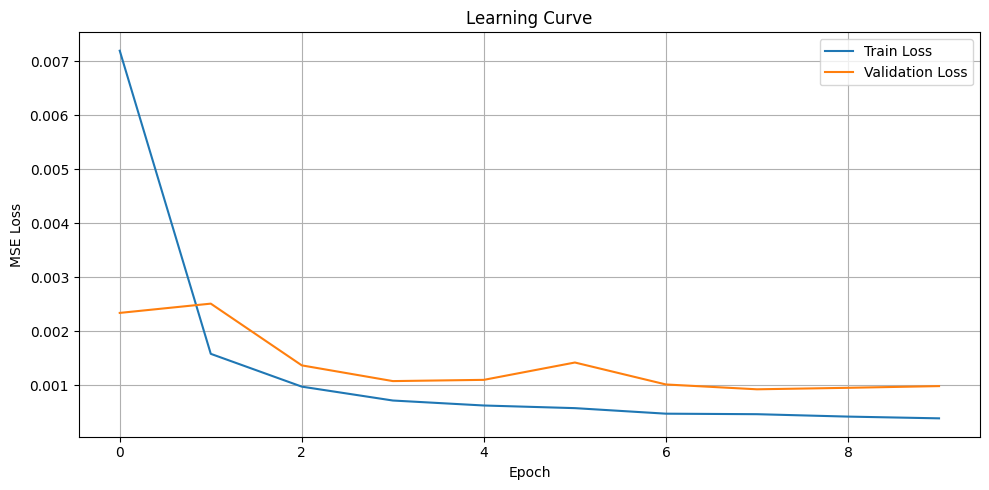
\includegraphics[width=1.0\textwidth]{learningCurveforCNN.png} % Adjust path and size
    \caption{Learning Curve for CNN model using ResNet18 for 10 epochs}
    \label{fig:learningCurveforCNN}
\end{figure}

\subsubsection{Quantitative Results}

As shown in Figure~\ref{fig:learningCurveforCNN}, the CNN model shows a significant improvement over the baseline model. 
The training loss began at around 0.007 and decreased sharply to around 0.0015 by epoch 1, then steadily decreased to around 0.0005 by the final 
epoch. This indicates that the model is learning effectively from the training data. 
We also see that the validation loss started near 0.0024 an over the 10 epochs decreased to 0.001, showing good generalization with minimal overfitting.
The small gaps between the training and validation loss after epoch 1, show that the model is performing well on both training and unseen data.


\subsubsection{Qualitative Results}

When running the CNN model in the CARLA simulator, the car exhibited significantly improved driving behavior compared to the baseline model. 
The car was able to navigate complex turns and maintain lane discipline more effectively. The model was able to make lane changes, and stay within its respective lane.
Similar to the baseline, the model struggles when it comes to large turns, but it does a better job staying away from walls and other obstacles.


\subsubsection{Challenges and Observations}

One key challenge was in the integration of image and turn signal data in a single model. This required tensor dimension reshaping and matching in PyTorch correctly, specifically in concatenating CNN-extracted features with scalar turn signal input. Mistakes here led to early runtime errors that had to be painstakingly debugged.
There was also the problem of generalization tracking. As training loss kept improving, validation loss began to plateau from epoch 6 onward, indicating the possibility of overfitting. This indicates the need for early stopping or regularization in subsequent models.


One key finding is that the CNN model performs much better than the baseline model, especially on examples where there are lane markings. The CNN learned to recognize helpful spatial features from the driving environment, resulting in smoother and more accurate steering and improved lane-keeping behavior at test time. 

\section{Conclusion}

Our ResNet18 model outperformed the ridge regression baseline, keeping the car in its lane more reliably and 
cutting validation loss by a noticeable margin. To build on this, we’ll introduce stronger data augmentation like MixUp or 
CutMix so the network learns to ignore odd artifacts and lighting changes. We also want to experiment with newer backbones 
such as EfficientNetV2 or Vision Transformers and try combining several models in an ensemble to cover each other’s weaknesses. 
Finally, more hyperparameter tuning based on the dataset collected from CARLA should help the model pick up 
driving‑specific features. 
These updates should lead to smoother steering on tight turns and better handling of roads the model hasn’t seen before.
\label{last_page}

\end{document}
